% Options for packages loaded elsewhere
\PassOptionsToPackage{unicode}{hyperref}
\PassOptionsToPackage{hyphens}{url}
%
\documentclass[
]{article}
\usepackage{lmodern}
\usepackage{amssymb,amsmath}
\usepackage{ifxetex,ifluatex}
\ifnum 0\ifxetex 1\fi\ifluatex 1\fi=0 % if pdftex
  \usepackage[T1]{fontenc}
  \usepackage[utf8]{inputenc}
  \usepackage{textcomp} % provide euro and other symbols
\else % if luatex or xetex
  \usepackage{unicode-math}
  \defaultfontfeatures{Scale=MatchLowercase}
  \defaultfontfeatures[\rmfamily]{Ligatures=TeX,Scale=1}
\fi
% Use upquote if available, for straight quotes in verbatim environments
\IfFileExists{upquote.sty}{\usepackage{upquote}}{}
\IfFileExists{microtype.sty}{% use microtype if available
  \usepackage[]{microtype}
  \UseMicrotypeSet[protrusion]{basicmath} % disable protrusion for tt fonts
}{}
\makeatletter
\@ifundefined{KOMAClassName}{% if non-KOMA class
  \IfFileExists{parskip.sty}{%
    \usepackage{parskip}
  }{% else
    \setlength{\parindent}{0pt}
    \setlength{\parskip}{6pt plus 2pt minus 1pt}}
}{% if KOMA class
  \KOMAoptions{parskip=half}}
\makeatother
\usepackage{xcolor}
\IfFileExists{xurl.sty}{\usepackage{xurl}}{} % add URL line breaks if available
\IfFileExists{bookmark.sty}{\usepackage{bookmark}}{\usepackage{hyperref}}
\hypersetup{
  pdftitle={Survey of Overall Election Employed by the Conservative Party},
  pdfauthor={Zhendong Zhang},
  hidelinks,
  pdfcreator={LaTeX via pandoc}}
\urlstyle{same} % disable monospaced font for URLs
\usepackage[margin=1in]{geometry}
\usepackage{color}
\usepackage{fancyvrb}
\newcommand{\VerbBar}{|}
\newcommand{\VERB}{\Verb[commandchars=\\\{\}]}
\DefineVerbatimEnvironment{Highlighting}{Verbatim}{commandchars=\\\{\}}
% Add ',fontsize=\small' for more characters per line
\usepackage{framed}
\definecolor{shadecolor}{RGB}{248,248,248}
\newenvironment{Shaded}{\begin{snugshade}}{\end{snugshade}}
\newcommand{\AlertTok}[1]{\textcolor[rgb]{0.94,0.16,0.16}{#1}}
\newcommand{\AnnotationTok}[1]{\textcolor[rgb]{0.56,0.35,0.01}{\textbf{\textit{#1}}}}
\newcommand{\AttributeTok}[1]{\textcolor[rgb]{0.77,0.63,0.00}{#1}}
\newcommand{\BaseNTok}[1]{\textcolor[rgb]{0.00,0.00,0.81}{#1}}
\newcommand{\BuiltInTok}[1]{#1}
\newcommand{\CharTok}[1]{\textcolor[rgb]{0.31,0.60,0.02}{#1}}
\newcommand{\CommentTok}[1]{\textcolor[rgb]{0.56,0.35,0.01}{\textit{#1}}}
\newcommand{\CommentVarTok}[1]{\textcolor[rgb]{0.56,0.35,0.01}{\textbf{\textit{#1}}}}
\newcommand{\ConstantTok}[1]{\textcolor[rgb]{0.00,0.00,0.00}{#1}}
\newcommand{\ControlFlowTok}[1]{\textcolor[rgb]{0.13,0.29,0.53}{\textbf{#1}}}
\newcommand{\DataTypeTok}[1]{\textcolor[rgb]{0.13,0.29,0.53}{#1}}
\newcommand{\DecValTok}[1]{\textcolor[rgb]{0.00,0.00,0.81}{#1}}
\newcommand{\DocumentationTok}[1]{\textcolor[rgb]{0.56,0.35,0.01}{\textbf{\textit{#1}}}}
\newcommand{\ErrorTok}[1]{\textcolor[rgb]{0.64,0.00,0.00}{\textbf{#1}}}
\newcommand{\ExtensionTok}[1]{#1}
\newcommand{\FloatTok}[1]{\textcolor[rgb]{0.00,0.00,0.81}{#1}}
\newcommand{\FunctionTok}[1]{\textcolor[rgb]{0.00,0.00,0.00}{#1}}
\newcommand{\ImportTok}[1]{#1}
\newcommand{\InformationTok}[1]{\textcolor[rgb]{0.56,0.35,0.01}{\textbf{\textit{#1}}}}
\newcommand{\KeywordTok}[1]{\textcolor[rgb]{0.13,0.29,0.53}{\textbf{#1}}}
\newcommand{\NormalTok}[1]{#1}
\newcommand{\OperatorTok}[1]{\textcolor[rgb]{0.81,0.36,0.00}{\textbf{#1}}}
\newcommand{\OtherTok}[1]{\textcolor[rgb]{0.56,0.35,0.01}{#1}}
\newcommand{\PreprocessorTok}[1]{\textcolor[rgb]{0.56,0.35,0.01}{\textit{#1}}}
\newcommand{\RegionMarkerTok}[1]{#1}
\newcommand{\SpecialCharTok}[1]{\textcolor[rgb]{0.00,0.00,0.00}{#1}}
\newcommand{\SpecialStringTok}[1]{\textcolor[rgb]{0.31,0.60,0.02}{#1}}
\newcommand{\StringTok}[1]{\textcolor[rgb]{0.31,0.60,0.02}{#1}}
\newcommand{\VariableTok}[1]{\textcolor[rgb]{0.00,0.00,0.00}{#1}}
\newcommand{\VerbatimStringTok}[1]{\textcolor[rgb]{0.31,0.60,0.02}{#1}}
\newcommand{\WarningTok}[1]{\textcolor[rgb]{0.56,0.35,0.01}{\textbf{\textit{#1}}}}
\usepackage{graphicx,grffile}
\makeatletter
\def\maxwidth{\ifdim\Gin@nat@width>\linewidth\linewidth\else\Gin@nat@width\fi}
\def\maxheight{\ifdim\Gin@nat@height>\textheight\textheight\else\Gin@nat@height\fi}
\makeatother
% Scale images if necessary, so that they will not overflow the page
% margins by default, and it is still possible to overwrite the defaults
% using explicit options in \includegraphics[width, height, ...]{}
\setkeys{Gin}{width=\maxwidth,height=\maxheight,keepaspectratio}
% Set default figure placement to htbp
\makeatletter
\def\fps@figure{htbp}
\makeatother
\setlength{\emergencystretch}{3em} % prevent overfull lines
\providecommand{\tightlist}{%
  \setlength{\itemsep}{0pt}\setlength{\parskip}{0pt}}
\setcounter{secnumdepth}{-\maxdimen} % remove section numbering

\title{Survey of Overall Election Employed by the Conservative Party}
\author{Zhendong Zhang}
\date{2020-10-2}

\begin{document}
\maketitle

\hypertarget{executive-summary}{%
\subsection{Executive Summary}\label{executive-summary}}

Nearly all political action committees, city council members, political
consultants, school board districts, government agencies, rely on
offline or online surveys to get the insights they need to drive their
causes and run quick polls on hot-button issues.

The importance of investigation is self-evident, and a good polling
update of investigation must not only reflect the reality, but also help
political parties adjust the focus of their campaign activities and
achieve more election goals within a limited budget.

Throughout the report, I was employed by the Conservative Party to
complete the following tasks:

\begin{enumerate}
\def\labelenumi{\arabic{enumi}.}
\item
  Based on the entire election environment, analyze the significance of
  the research report and promote it to a wide range of application
  scenarios, which can help customers understand the significance of the
  survey;
\item
  Design the questionnaire based on the survey method and put it to the
  target people in different forms, which will help the survey designer
  to obtain data;
\item
  Data analysis based on the simulation results, which can verify the
  correctness of the method;
\item
  Discuss possible biases and errors in the questionnaire and study how
  they affect the results of the survey, which will show us the things
  behind the election;
\item
  Display the methods and references used in the entire report in the
  report.
\end{enumerate}

\hypertarget{introduction}{%
\subsection{Introduction}\label{introduction}}

The whole polling status updating is a survey of how I conduct this
research to help our client, that is, the Conservative.

Focusing on present\textsuperscript{1}, the Liberals hold a comfortable
lead in Atlantic Canada and are ahead of the Conservatives in British
Columbia. Two-thirds of the Liberals' seat advantage nationwide is due
to Ontario, where the party has a lead over the Conservatives. The
Liberals are also narrowly in front of the Bloc in Quebec. The
Conservatives are solidly in first in Alberta and the Prairies. Both the
NDP and the Greens have their strongest results in B.C.

When designing the questions and conducting the survey, all the work
should be put into certain context. We can use survey to identify
supporters for campaign, gather feedback from constituents, organize
rallies(or potential rallies), get feedback of present political event,
help the winning local election.

Also the code for this post is in the Git Repo:
\url{https://github.com/Craymate/Survey-Election}

\hypertarget{survey-methodology}{%
\subsection{Survey Methodology}\label{survey-methodology}}

When employed by certain political party, writing clear and neutral
survey questions is not easy like it seems. There's more survey
methodology to demystify when conducting our research, and the question
wording is important too.

\hypertarget{survey-objections}{%
\subsubsection{Survey Objections}\label{survey-objections}}

The object of the survey is:

\begin{enumerate}
\def\labelenumi{\arabic{enumi}.}
\item
  To find out the main supporters and get contact.
\item
  To get feedback of different local districts and find their focal
  point including what they want to keep most and what they want to
  change most.
\item
  To find room to increase votes and help make real-time adjustments to
  policies.
\end{enumerate}

\hypertarget{sample-frames-and-methodology}{%
\subsubsection{Sample Frames and
Methodology}\label{sample-frames-and-methodology}}

\begin{enumerate}
\def\labelenumi{\arabic{enumi}.}
\item
  This survey aims at all civilizations in Canada, so we can get
  information from all districts and use differences between districts
  to help political parties make customized decisions.
\item
  This survey use online and offline survey methods are used to
  distribute questionnaires in public places with equal probability and
  random sampling, which is usually called Simple Random Sampling
  Without Replacement (SRSWOR)\textsuperscript{2}, and the
  questionnaires are distributed on the Internet using a neutral
  platform.
\end{enumerate}

\hypertarget{relevant-data-colletion}{%
\subsubsection{Relevant Data Colletion}\label{relevant-data-colletion}}

In the process of designing the questionnaire, it is necessary to design
``irrelevant questions'' that are different from the target question to
help the data analyst classify the sample, or analyze whether the
collected sample is valid. This often includes:

\begin{enumerate}
\def\labelenumi{\arabic{enumi}.}
\item
  Gender and age (or even occupation), data analysts usually need to
  ensure that the questionnaire is distributed to all types of people.
\item
  Simple daily questions. When questionnaire collectors find that
  subjects have abnormal answers to such questions, they can usually
  screen out invalid questionnaires during the result entry process.
\end{enumerate}

\hypertarget{accuracy-estimation}{%
\subsubsection{Accuracy Estimation}\label{accuracy-estimation}}

The parameter estimates obtained by sampling are usually biased. Part of
this bias comes from the cognitive bias of the subjects on the same
question, and part comes from the bias in the questionnaire design. In
particular:

\begin{enumerate}
\def\labelenumi{\arabic{enumi}.}
\item
  The position of the questionnaire designer will affect the design of
  the questionnaire and lead to deviations;
\item
  The order of the questions may induce participants to answer an
  important question from a certain angle (what the questionnaire
  designer hopes to get). In this way, using prejudice to induce
  participants to answer will often get ``good'' results but cannot
  affect the votes of neutrals in the long term, because they are also
  susceptible to other information interference. At the same time, it
  will also cause the political parties to produce miscalculations on
  the situation and thus formulate wrong campaign strategies.
\end{enumerate}

\hypertarget{reach-respondents-and-dealing-with-non-response}{%
\subsubsection{Reach Respondents and Dealing with
Non-response}\label{reach-respondents-and-dealing-with-non-response}}

In fact, dealing with Non-responses is the same thing as finding the
target respondents. The length of the questionnaire (number of
questions), the text layout of the question, and even the environment
under which the survey is conducted will affect the quality of the
questionnaire, which increases the probability of Non-responses and
reduces the probability of obtaining target information.

In the Internet space, in order to obtain higher-quality sample
information, the usual methods are to select groups or individuals that
they trust to conduct surveys, or to issue questionnaires on platforms
that they are familiar with daily. But usually this approach has strong
prejudices. For example, we know that the in-depth users of different
social platforms often have very big differences in group
characteristics from the ``popular'' we want to investigate, and the
similarity between relatives and friends is even greater. It violates
the principle of medium probability of the interviewee in the entire
target group.

To sum up, in order to ensure the unbiased and effective sampling, we
choose to put the number of questionnaires based on the proportion of
users on different social software, and choose different public places
to put questionnaires commensurate with the proportion of people flow,
which use the stratified sampling method.

\hypertarget{cost-estimation}{%
\subsubsection{Cost estimation}\label{cost-estimation}}

Regardless of whether it is filled online or offline, we will give
participants an incentive ranging from \$1-100 (the higher the bonus,
the lower the probability of obtaining), and the dairy products of brand
A (virtual brand) or B Daily cleaning appliances of the brand (virtual
brand) are given as incentives to raise sponsorship as the funding for
this survey. After conversion, it can be considered that there is no
actual net expenditure in this survey.

\hypertarget{privacy-protection}{%
\subsubsection{Privacy Protection}\label{privacy-protection}}

Sometimes researchers are confused about how to determine what
information is private. Subject's privacy protection is an important
means and ethical requirement for obtaining target information, and
behaviors that respect privacy often bring more votes and favors to
political parties (except for individuals who advocate that the
government should obtain more citizens' information).

\hypertarget{survey-design}{%
\subsection{Survey Design}\label{survey-design}}

\hypertarget{motivation}{%
\subsubsection{Motivation}\label{motivation}}

Our client, the Conservative, is left behind the election polling. After
the selection of our new leader, we got a small bump but that is not
enough. We need to ensure that the Liberals won't get majority seats and
fight for potential leading.

Based on the above methodology and basic guidelines that need to be paid
attention to, I designed the following questionnaire:

\hypertarget{fundamental-question}{%
\subsubsection{Fundamental Question}\label{fundamental-question}}

\begin{enumerate}
\def\labelenumi{(\arabic{enumi})}
\item
  How did you know about this survey?(Written by Questionnaire
  Collector)
\item
  Are you eligible to vote?(choose Y or N)
\item
  Which province are you located?(Use province code and option not to
  say)
\item
  What is your gender?(Open question)
\item
  How old are you?(Open question)
\end{enumerate}

\hypertarget{trap-questionvalidity-checking}{%
\subsubsection{Trap question(Validity
Checking)}\label{trap-questionvalidity-checking}}

\begin{enumerate}
\def\labelenumi{(\arabic{enumi})}
\setcounter{enumi}{5}
\item
  In this question, please choose A(Give choices of A and B)
\item
  In this question, please choose F(Give choices of T and F)
\end{enumerate}

\hypertarget{current-hotspot-affairs}{%
\subsubsection{Current Hotspot Affairs}\label{current-hotspot-affairs}}

\begin{enumerate}
\def\labelenumi{(\arabic{enumi})}
\setcounter{enumi}{7}
\item
  Do you think it is necessary to further strengthen or maintain the
  control of public areas such as bars?(Give choices of Yes and No)
\item
  Do you think it is necessary to further postpone the opening of
  school?(Give choices of Yes and No)
\item
  Do you think it is necessary to increase the minimum monthly income
  limit in CRB?(Give choices of Yes and No)
\item
  Score from 1 to 10, how do you think the government should balance the
  promotion of vaccine trials and safety tests (the larger the value,
  the more important the safety test is)
\item
  On a scale from 1 to 10, how do you think the government should make
  trade-offs between promoting the resumption of work and production and
  restricting production to ensure safety (the bigger the
  representative, the more hopeful it is to resume working)
\end{enumerate}

\hypertarget{political-orientation-issues}{%
\subsubsection{Political orientation
issues}\label{political-orientation-issues}}

\begin{enumerate}
\def\labelenumi{(\arabic{enumi})}
\setcounter{enumi}{12}
\item
  At present, which party would you vote?(Give choices and option not to
  say)
\item
  Which party you think will win the election?(Give choices)
\item
  Which party you think will get majority seats?(Give choices)
\end{enumerate}

\hypertarget{simulating}{%
\subsection{Simulating}\label{simulating}}

In this part, I generated 10,000 questionnaires after screening, which
means that there are no vacancies in the sample data that answered the
trap questions correctly. In issues that are not related to political
bias, the data generated is as even as possible.

\begin{Shaded}
\begin{Highlighting}[]
\NormalTok{n=}\FloatTok{1e4}
\KeywordTok{set.seed}\NormalTok{(}\DecValTok{1}\NormalTok{)}
\NormalTok{dat <-}\StringTok{ }\KeywordTok{data.frame}\NormalTok{(}
  \DataTypeTok{platform=}\KeywordTok{rep}\NormalTok{(}\KeywordTok{c}\NormalTok{(}\StringTok{'Park'}\NormalTok{,}\StringTok{'Metro'}\NormalTok{,}\StringTok{'Busstop'}\NormalTok{,}\StringTok{'Playground'}\NormalTok{,}\StringTok{'Twitter'}\NormalTok{,}\StringTok{'Facebook'}\NormalTok{,}\StringTok{'Reddit'}\NormalTok{,}\StringTok{'Quora'}\NormalTok{),}\DecValTok{125}\NormalTok{),}
  \DataTypeTok{eligible=}\KeywordTok{rep}\NormalTok{(}\StringTok{'Y'}\NormalTok{,n),}
  \DataTypeTok{province=}\KeywordTok{c}\NormalTok{(}\KeywordTok{rep}\NormalTok{(}\KeywordTok{c}\NormalTok{(}\StringTok{'ON'}\NormalTok{,}\StringTok{'QC'}\NormalTok{,}\StringTok{'PE'}\NormalTok{,}\StringTok{'BC'}\NormalTok{,}\StringTok{'NB'}\NormalTok{,}\StringTok{'NS'}\NormalTok{,}\StringTok{'MB'}\NormalTok{,}\StringTok{'NL'}\NormalTok{,}\StringTok{'SK'}\NormalTok{,}\StringTok{'AB'}\NormalTok{,}\StringTok{'YT'}\NormalTok{,}\StringTok{'NT'}\NormalTok{,}\StringTok{'NU'}\NormalTok{),}\DecValTok{769}\NormalTok{),}\KeywordTok{rep}\NormalTok{(}\StringTok{'prefer_not_say'}\NormalTok{,}\DecValTok{3}\NormalTok{)),}
  \DataTypeTok{gender=}\KeywordTok{rep}\NormalTok{(}\KeywordTok{c}\NormalTok{(}\StringTok{'M'}\NormalTok{,}\StringTok{'F'}\NormalTok{),}\DecValTok{5000}\NormalTok{),}
  \DataTypeTok{age=}\KeywordTok{sample}\NormalTok{(}\DecValTok{20}\OperatorTok{:}\DecValTok{60}\NormalTok{,}\DecValTok{10000}\NormalTok{,}\DataTypeTok{replace =}\NormalTok{ T),}
  \DataTypeTok{trapa=}\KeywordTok{rep}\NormalTok{(}\StringTok{'A'}\NormalTok{,}\FloatTok{1e4}\NormalTok{),}
  \DataTypeTok{trapf=}\KeywordTok{rep}\NormalTok{(}\StringTok{'F'}\NormalTok{,}\FloatTok{1e4}\NormalTok{),}
  \DataTypeTok{pub_ctrl=}\KeywordTok{sample}\NormalTok{(}\KeywordTok{c}\NormalTok{(}\StringTok{'Y'}\NormalTok{,}\StringTok{'N'}\NormalTok{),}\DecValTok{10000}\NormalTok{,}\DataTypeTok{replace =}\NormalTok{ T,}\DataTypeTok{prob =} \KeywordTok{c}\NormalTok{(}\FloatTok{0.3}\NormalTok{,}\FloatTok{0.7}\NormalTok{)),}
  \DataTypeTok{sch_open=}\KeywordTok{sample}\NormalTok{(}\KeywordTok{c}\NormalTok{(}\StringTok{'Y'}\NormalTok{,}\StringTok{'N'}\NormalTok{),}\DecValTok{10000}\NormalTok{,}\DataTypeTok{replace =}\NormalTok{ T,}\DataTypeTok{prob =} \KeywordTok{c}\NormalTok{(}\FloatTok{0.35}\NormalTok{,}\FloatTok{0.65}\NormalTok{)),}
  \DataTypeTok{min_inc=}\KeywordTok{sample}\NormalTok{(}\KeywordTok{c}\NormalTok{(}\StringTok{'Y'}\NormalTok{,}\StringTok{'N'}\NormalTok{),}\DecValTok{10000}\NormalTok{,}\DataTypeTok{replace =}\NormalTok{ T,}\DataTypeTok{prob =} \KeywordTok{c}\NormalTok{(}\FloatTok{0.8}\NormalTok{,}\FloatTok{0.2}\NormalTok{)),}
  \DataTypeTok{balance1 =} \KeywordTok{as.integer}\NormalTok{(}\KeywordTok{rnorm}\NormalTok{(}\DecValTok{10000}\NormalTok{,}\FloatTok{5.5}\NormalTok{,}\DecValTok{1}\NormalTok{)),}
  \DataTypeTok{balance2 =} \KeywordTok{as.integer}\NormalTok{(}\KeywordTok{rnorm}\NormalTok{(}\DecValTok{10000}\NormalTok{,}\FloatTok{5.5}\NormalTok{,}\FloatTok{1.2}\NormalTok{)),}
  \DataTypeTok{vote =} \KeywordTok{sample}\NormalTok{(}\KeywordTok{c}\NormalTok{(}\StringTok{'LIB'}\NormalTok{,}\StringTok{'CON'}\NormalTok{,}\StringTok{'NDP'}\NormalTok{,}\StringTok{'BQ'}\NormalTok{,}\StringTok{'GRN'}\NormalTok{,}\StringTok{'OTH'}\NormalTok{),}\DecValTok{10000}\NormalTok{,}\DataTypeTok{replace =}\NormalTok{ T,}\DataTypeTok{prob =} \KeywordTok{c}\NormalTok{(}\FloatTok{0.364}\NormalTok{,}\FloatTok{0.309}\NormalTok{,}\FloatTok{0.173}\NormalTok{,}\FloatTok{0.067}\NormalTok{,}\FloatTok{0.061}\NormalTok{,}\FloatTok{0.026}\NormalTok{)),}
  \DataTypeTok{win =} \KeywordTok{sample}\NormalTok{(}\KeywordTok{c}\NormalTok{(}\StringTok{'LIB'}\NormalTok{,}\StringTok{'CON'}\NormalTok{,}\StringTok{'NDP'}\NormalTok{),}\DecValTok{10000}\NormalTok{,}\DataTypeTok{replace =}\NormalTok{ T,}\DataTypeTok{prob =} \KeywordTok{c}\NormalTok{(}\FloatTok{0.6}\NormalTok{,}\FloatTok{0.3}\NormalTok{,}\FloatTok{0.1}\NormalTok{)),}
  \DataTypeTok{majority =} \KeywordTok{sample}\NormalTok{(}\KeywordTok{c}\NormalTok{(}\StringTok{'LIB'}\NormalTok{,}\StringTok{'CON'}\NormalTok{),}\DecValTok{10000}\NormalTok{,}\DataTypeTok{replace =}\NormalTok{ T,}\DataTypeTok{prob =} \KeywordTok{c}\NormalTok{(}\FloatTok{0.85}\NormalTok{,}\FloatTok{0.15}\NormalTok{)),}
  \DataTypeTok{stringsAsFactors =}\NormalTok{ T}
\NormalTok{)}
\end{Highlighting}
\end{Shaded}

and we can get our simulated data frame in an ideal state.

\hypertarget{results}{%
\subsection{Results}\label{results}}

Although the result comes from simulating, we should know what matters
is the method of analysis, not the result of a particular survey.

\hypertarget{fundamental-summary}{%
\subsubsection{Fundamental Summary}\label{fundamental-summary}}

First we can view the basic information of the data set generated by the
simulation:

\begin{Shaded}
\begin{Highlighting}[]
\CommentTok{# show structure}
\KeywordTok{str}\NormalTok{(dat)}
\end{Highlighting}
\end{Shaded}

\begin{verbatim}
## 'data.frame':    10000 obs. of  15 variables:
##  $ platform: Factor w/ 8 levels "Busstop","Facebook",..: 4 3 1 5 8 2 7 6 4 3 ...
##  $ eligible: Factor w/ 1 level "Y": 1 1 1 1 1 1 1 1 1 1 ...
##  $ province: Factor w/ 14 levels "AB","BC","MB",..: 9 12 10 2 4 6 3 5 13 1 ...
##  $ gender  : Factor w/ 2 levels "F","M": 2 1 2 1 2 1 2 1 2 1 ...
##  $ age     : int  23 58 20 53 42 33 37 52 40 40 ...
##  $ trapa   : Factor w/ 1 level "A": 1 1 1 1 1 1 1 1 1 1 ...
##  $ trapf   : Factor w/ 1 level "F": 1 1 1 1 1 1 1 1 1 1 ...
##  $ pub_ctrl: Factor w/ 2 levels "N","Y": 1 1 2 1 1 2 1 1 2 1 ...
##  $ sch_open: Factor w/ 2 levels "N","Y": 1 1 2 1 1 1 2 1 2 1 ...
##  $ min_inc : Factor w/ 2 levels "N","Y": 2 2 2 2 2 2 2 1 2 2 ...
##  $ balance1: int  6 4 3 6 5 6 6 5 4 5 ...
##  $ balance2: int  6 4 5 6 4 5 4 5 5 5 ...
##  $ vote    : Factor w/ 6 levels "BQ","CON","GRN",..: 4 1 4 2 3 4 1 4 4 4 ...
##  $ win     : Factor w/ 3 levels "CON","LIB","NDP": 2 3 1 2 2 2 2 1 2 2 ...
##  $ majority: Factor w/ 2 levels "CON","LIB": 2 2 2 2 1 2 2 2 2 2 ...
\end{verbatim}

\begin{Shaded}
\begin{Highlighting}[]
\CommentTok{# brief summary}
\KeywordTok{summary}\NormalTok{(dat)}
\end{Highlighting}
\end{Shaded}

\begin{verbatim}
##        platform    eligible     province    gender        age       trapa    
##  Busstop   :1250   Y:10000   AB     : 769   F:5000   Min.   :20.0   A:10000  
##  Facebook  :1250             BC     : 769   M:5000   1st Qu.:30.0            
##  Metro     :1250             MB     : 769            Median :40.0            
##  Park      :1250             NB     : 769            Mean   :39.9            
##  Playground:1250             NL     : 769            3rd Qu.:50.0            
##  Quora     :1250             NS     : 769            Max.   :60.0            
##  (Other)   :2500             (Other):5386                                    
##  trapf     pub_ctrl sch_open min_inc     balance1        balance2    
##  F:10000   N:7041   N:6471   N:1934   Min.   :1.000   Min.   :0.000  
##            Y:2959   Y:3529   Y:8066   1st Qu.:4.000   1st Qu.:4.000  
##                                       Median :5.000   Median :5.000  
##                                       Mean   :5.008   Mean   :4.992  
##                                       3rd Qu.:6.000   3rd Qu.:6.000  
##                                       Max.   :9.000   Max.   :9.000  
##                                                                      
##   vote       win       majority  
##  BQ : 699   CON:2999   CON:1423  
##  CON:3059   LIB:6044   LIB:8577  
##  GRN: 582   NDP: 957             
##  LIB:3643                        
##  NDP:1757                        
##  OTH: 260                        
## 
\end{verbatim}

\hypertarget{exploratory-analysis}{%
\subsubsection{Exploratory Analysis}\label{exploratory-analysis}}

Using the fundamental information of survey results, it's not intuitive
for our clients. So we hope to reflect the exact relationship through
quantitative expression, in this section, we are trying to find out if
the two numeric \texttt{balance} answers can influence each other.

\begin{Shaded}
\begin{Highlighting}[]
\CommentTok{# correlation statistics}
\KeywordTok{cor}\NormalTok{(dat}\OperatorTok{$}\NormalTok{balance1, dat}\OperatorTok{$}\NormalTok{balance2)}
\end{Highlighting}
\end{Shaded}

\begin{verbatim}
## [1] 0.001885394
\end{verbatim}

\begin{Shaded}
\begin{Highlighting}[]
\CommentTok{# linear regression}
\NormalTok{linear.model1 <-}\StringTok{ }\KeywordTok{lm}\NormalTok{(balance1 }\OperatorTok{~}\StringTok{ }\NormalTok{balance2,}
                    \DataTypeTok{data =}\NormalTok{ dat)}
\KeywordTok{summary}\NormalTok{(linear.model1)}
\end{Highlighting}
\end{Shaded}

\begin{verbatim}
## 
## Call:
## lm(formula = balance1 ~ balance2, data = dat)
## 
## Residuals:
##     Min      1Q  Median      3Q     Max 
## -4.0098 -1.0066 -0.0082  0.9902  3.9934 
## 
## Coefficients:
##             Estimate Std. Error t value Pr(>|t|)    
## (Intercept) 5.000329   0.043041 116.176   <2e-16 ***
## balance2    0.001577   0.008363   0.189     0.85    
## ---
## Signif. codes:  0 '***' 0.001 '**' 0.01 '*' 0.05 '.' 0.1 ' ' 1
## 
## Residual standard error: 1.045 on 9998 degrees of freedom
## Multiple R-squared:  3.555e-06,  Adjusted R-squared:  -9.646e-05 
## F-statistic: 0.03554 on 1 and 9998 DF,  p-value: 0.8505
\end{verbatim}

From the statistics and also the summary, it's significant that there's
no linear correlation between this two variables. This result comes from
our simulation, so of course nothing will be discovered. But in some
circumstances, some kind of linear dependence exists between two numeric
variables, and our clients can use such model to develop or modify
policies.

Moreover, there are more \texttt{factor} variables we need to analyze.
And what we do next is to test whether the means of the two types of
samples are the same.

To be precise, we want to do a hypothesis test, that is, whether people
of different genders will make the same level in the first balancing
decision (here we are based on the estimation method of statistics in
sampling theory, and we believe that the mean can reflect unbiasedly
Average) decision-making.

So our original hypothesis is: Different genders have the same level of
response to the first type of balanced decision-making. In contrast, the
alternative hypothesis is that different genders have different levels
of response to the first type of balanced decision-making.

\begin{Shaded}
\begin{Highlighting}[]
\NormalTok{a <-}\StringTok{ }\NormalTok{dat}\OperatorTok{$}\NormalTok{balance1[}\KeywordTok{which}\NormalTok{(dat}\OperatorTok{$}\NormalTok{gender}\OperatorTok{==}\StringTok{'M'}\NormalTok{)]}
\NormalTok{b <-}\StringTok{ }\NormalTok{dat}\OperatorTok{$}\NormalTok{balance1[}\KeywordTok{which}\NormalTok{(dat}\OperatorTok{$}\NormalTok{gender}\OperatorTok{==}\StringTok{'F'}\NormalTok{)]}

\KeywordTok{t.test}\NormalTok{(a,b)}
\end{Highlighting}
\end{Shaded}

\begin{verbatim}
## 
##  Welch Two Sample t-test
## 
## data:  a and b
## t = -0.66977, df = 9995.7, p-value = 0.503
## alternative hypothesis: true difference in means is not equal to 0
## 95 percent confidence interval:
##  -0.05497341  0.02697341
## sample estimates:
## mean of x mean of y 
##    5.0012    5.0152
\end{verbatim}

After testing, we found that the two groups of people did have the same
decision-making level in the first balanced decision. That is, after
testing, according to the statistics and p-value, the mean values of the
two numerical variables are the same, so here we accept the null
hypothesis and consider that they are different The genders have the
same level of response to the first type of balanced decision-making.

Indeed, this result is produced because the result data set is generated
by our use of the program, rather than a response to the real situation.
But at the same time we need to know that different groups of people,
especially groups with large differences in group characteristics,
usually have different levels of group responses when facing problems,
and political parties (or other customers) need to use this group
difference to obtain specific groups. Stable support, and to a greater
extent strive for the favor of opposing groups to prevent them from
falling to competitors.

\hypertarget{visual-analysis-method}{%
\subsubsection{Visual analysis method}\label{visual-analysis-method}}

The intuitive feeling comes from the persuasive chart. Below we tried
different methods to try to characterize the result data:

\hypertarget{preparing}{%
\paragraph{Preparing}\label{preparing}}

\begin{Shaded}
\begin{Highlighting}[]
\CommentTok{# load packages}
\KeywordTok{library}\NormalTok{(ggplot2)}
\KeywordTok{library}\NormalTok{(plyr)}
\KeywordTok{library}\NormalTok{(olsrr)}
\end{Highlighting}
\end{Shaded}

\begin{verbatim}
## 
## Attaching package: 'olsrr'
\end{verbatim}

\begin{verbatim}
## The following object is masked from 'package:datasets':
## 
##     rivers
\end{verbatim}

\hypertarget{bar-plot}{%
\paragraph{Bar plot}\label{bar-plot}}

When we look at the distribution of platform, we can use \texttt{table}
to generate result like this:

\begin{Shaded}
\begin{Highlighting}[]
\KeywordTok{table}\NormalTok{(dat}\OperatorTok{$}\NormalTok{platform)}
\end{Highlighting}
\end{Shaded}

\begin{verbatim}
## 
##    Busstop   Facebook      Metro       Park Playground      Quora     Reddit 
##       1250       1250       1250       1250       1250       1250       1250 
##    Twitter 
##       1250
\end{verbatim}

And we are going to visualize it like Figure 1 below:

\begin{Shaded}
\begin{Highlighting}[]
\NormalTok{num <-}\StringTok{ }\KeywordTok{as.numeric}\NormalTok{(}\KeywordTok{table}\NormalTok{(dat}\OperatorTok{$}\NormalTok{platform))}
\NormalTok{names <-}\StringTok{ }\KeywordTok{names}\NormalTok{(}\KeywordTok{table}\NormalTok{(dat}\OperatorTok{$}\NormalTok{platform))}
\NormalTok{df <-}\StringTok{ }\KeywordTok{data.frame}\NormalTok{(}\DataTypeTok{num=}\NormalTok{num,}\DataTypeTok{names=}\NormalTok{names)}

\KeywordTok{ggplot}\NormalTok{(df, }\KeywordTok{aes}\NormalTok{(}\DataTypeTok{x=}\NormalTok{names, }\DataTypeTok{y=}\NormalTok{num, }\DataTypeTok{fill=}\NormalTok{names)) }\OperatorTok{+}
\StringTok{  }\KeywordTok{geom_bar}\NormalTok{(}\DataTypeTok{stat=}\StringTok{"identity"}\NormalTok{)}\OperatorTok{+}\KeywordTok{theme_minimal}\NormalTok{() }\OperatorTok{+}
\StringTok{  }\KeywordTok{ggtitle}\NormalTok{(}\StringTok{'Figure 1: Sample Distribution of Platform'}\NormalTok{)}
\end{Highlighting}
\end{Shaded}

\begin{center}\includegraphics{Final_files/figure-latex/unnamed-chunk-7-1} \end{center}

\hypertarget{density-plot}{%
\paragraph{Density Plot}\label{density-plot}}

Studying the density distribution of two types of numerical samples can
compare the differences between the two types of samples at the same
level, and through the method of combination graphs, this comparison is
more intuitive:

\begin{Shaded}
\begin{Highlighting}[]
\CommentTok{# calculate mean}
\NormalTok{mu <-}\StringTok{ }\KeywordTok{ddply}\NormalTok{(dat, }\StringTok{"gender"}\NormalTok{, summarise, }\DataTypeTok{grp.mean=}\KeywordTok{mean}\NormalTok{(balance1))}
\CommentTok{# density plot}
\KeywordTok{ggplot}\NormalTok{(dat, }\KeywordTok{aes}\NormalTok{(}\DataTypeTok{x=}\NormalTok{balance1, }\DataTypeTok{color=}\NormalTok{gender)) }\OperatorTok{+}
\StringTok{  }\KeywordTok{geom_density}\NormalTok{()}\OperatorTok{+}
\StringTok{  }\KeywordTok{geom_vline}\NormalTok{(}\DataTypeTok{data=}\NormalTok{mu, }\KeywordTok{aes}\NormalTok{(}\DataTypeTok{xintercept=}\NormalTok{grp.mean, }\DataTypeTok{color=}\NormalTok{gender),}
             \DataTypeTok{linetype=}\StringTok{"dashed"}\NormalTok{)}\OperatorTok{+}
\StringTok{  }\KeywordTok{ggtitle}\NormalTok{(}\StringTok{'Figure 2: Density Plot of the first balance vote between genders'}\NormalTok{)}
\end{Highlighting}
\end{Shaded}

\begin{center}\includegraphics{Final_files/figure-latex/unnamed-chunk-8-1} \end{center}

Since we used simulated data for verification, we can find in Figure 2
that the two genders are the same on the image. But by observing the
fineness of the image, it can be found that the density map is indeed an
excellent visualization method.

\hypertarget{boxplot}{%
\paragraph{Boxplot}\label{boxplot}}

In addition to the density map that can reflect the overall nature, we
can also use box plots that can reflect the overall value distribution
to depict the performance of different variables or different
individuals of the same variable:

\hypertarget{different-variables}{%
\subparagraph{Different Variables}\label{different-variables}}

If we want to know the difference between the results of two balanced
votes, we can use:

\begin{Shaded}
\begin{Highlighting}[]
\NormalTok{df <-}\StringTok{ }\KeywordTok{data.frame}\NormalTok{(}\DataTypeTok{votes =} \KeywordTok{c}\NormalTok{(dat}\OperatorTok{$}\NormalTok{balance1,dat}\OperatorTok{$}\NormalTok{balance2),}
                 \DataTypeTok{tags =} \KeywordTok{c}\NormalTok{(}\KeywordTok{rep}\NormalTok{(}\StringTok{'V1'}\NormalTok{,}\FloatTok{5e3}\NormalTok{),}\KeywordTok{rep}\NormalTok{(}\StringTok{'V2'}\NormalTok{,}\FloatTok{5e3}\NormalTok{)))}

\KeywordTok{ggplot}\NormalTok{(df, }\KeywordTok{aes}\NormalTok{(}\DataTypeTok{x=}\NormalTok{tags, }\DataTypeTok{y=}\NormalTok{votes, }\DataTypeTok{fill=}\NormalTok{tags)) }\OperatorTok{+}
\StringTok{  }\KeywordTok{geom_boxplot}\NormalTok{() }\OperatorTok{+}
\StringTok{  }\KeywordTok{ggtitle}\NormalTok{(}\StringTok{'Figure 3: Boxplot Comparison of Two Variables'}\NormalTok{)}
\end{Highlighting}
\end{Shaded}

\begin{center}\includegraphics{Final_files/figure-latex/unnamed-chunk-9-1} \end{center}

The result Figure 3 also reflects the similarity of the two simulation
variables, which verifies the effectiveness of the method.

\hypertarget{one-variable-in-different-groups}{%
\subparagraph{One Variable in Different
Groups}\label{one-variable-in-different-groups}}

If we want to know the difference between the results of two balanced
groups, we can use:

\begin{Shaded}
\begin{Highlighting}[]
\KeywordTok{ggplot}\NormalTok{(dat, }\KeywordTok{aes}\NormalTok{(}\DataTypeTok{x=}\NormalTok{win, }\DataTypeTok{y=}\NormalTok{balance1, }\DataTypeTok{fill=}\NormalTok{win)) }\OperatorTok{+}
\StringTok{  }\KeywordTok{geom_boxplot}\NormalTok{() }\OperatorTok{+}
\StringTok{  }\KeywordTok{ggtitle}\NormalTok{(}\StringTok{'Figure 4: Boxplot Comparison of Two Groups in Balance 1'}\NormalTok{)}
\end{Highlighting}
\end{Shaded}

\begin{center}\includegraphics{Final_files/figure-latex/unnamed-chunk-10-1} \end{center}

Same as before, the result Figure 4 also reflects the similarity of the
simulation data of different groups.

\hypertarget{regression-plot}{%
\paragraph{Regression Plot}\label{regression-plot}}

Different from the previous drawing, here we use the regression model
established before for diagnosis, and use the diagnosis method in the
\texttt{olsrr} package to draw all the diagnostic images together.

\begin{Shaded}
\begin{Highlighting}[]
\KeywordTok{ols_plot_diagnostics}\NormalTok{(linear.model1)}
\end{Highlighting}
\end{Shaded}

\begin{center}\includegraphics{Final_files/figure-latex/unnamed-chunk-11-1} \end{center}

\begin{center}\includegraphics{Final_files/figure-latex/unnamed-chunk-11-2} \end{center}

\begin{center}\includegraphics{Final_files/figure-latex/unnamed-chunk-11-3} \end{center}

Looking at the figures, you can find that such a regression image can be
more useful in real application scenarios.

\hypertarget{discussion}{%
\subsection{Discussion}\label{discussion}}

\begin{enumerate}
\def\labelenumi{\arabic{enumi}.}
\tightlist
\item
  In this sampling survey and simulation process, are there still errors
  or biases?
\end{enumerate}

In such a sample survey, any form of prejudice and error are
unavoidable. For example: This simulation took an equal amount of
samples on each social platform, but in fact, the number of active
people on each platform is different and should be distributed in a
certain proportion. The same problem also appears in the sampling of
public places. Of course, different public places have different numbers
of active people.

The information collected does not fully reflect the real situation. For
example, due to factors such as incorrect filling or deliberate wrong
filling, not all subjects who claim to be eligible to vote have the
right to vote. This will also make it difficult to distinguish which
samples are indeed valid. We can only obtain more information. Samples
and unbiased estimates based on sampling theory to obtain as accurate
information as possible.

\begin{enumerate}
\def\labelenumi{\arabic{enumi}.}
\setcounter{enumi}{1}
\tightlist
\item
  In this sampling survey and simulation process, how can we help
  customers(the Conservative) through the results?
\end{enumerate}

Through the analysis of the results, we can indeed provide customers
with a lot of substantive and actionable suggestions. For example, the
quantitative methods and hypothesis testing methods used in the
``Results'' section can determine the source of stable support for
customers and the groups that need to be sought. By changing the means
of propaganda or the allocation of resources invested in elections, the
swing votes of a particular electoral district can be significantly
increased. These are specific practical suggestions

In addition, the results of the survey can help customers understand the
current situation and obtain more targeted results in further
investigations. Even if you don't dig deeper and use the visualization
methods of charts, you can intuitively show the results of the election
to your partners, win more support for yourself, and create stronger
propaganda capital.

\begin{enumerate}
\def\labelenumi{\arabic{enumi}.}
\setcounter{enumi}{2}
\tightlist
\item
  In this sampling survey and simulation process, what kind of result
  can be considered good?
\end{enumerate}

In the whole survey results, the authenticity and validity of the
results are two very important parts. According to sampling theory, a
survey result is considered a good survey only when it is true and
credible and contains more information.

First of all, ask yourself a question. Why is it not always a good thing
to support the majority of the party stations where customers are in the
survey results? How do you prove that your results are credible when
your survey results are very different from those done by others?

If you find friends who are close to your own ideas and conduct
provocative investigations in a small area, the results will of course
be very biased. A good survey should not mislead or influence the
concept of the surveyed, let alone select a specific group for the
survey, which will run counter to the purpose of the survey. The survey
is a non-interference one-to-many exchange. It is a friendly exchange of
information under the protection of respect and protection of the
privacy of the other party. Only when the surveyed person is not
selected outside the scope, the questionnaire should not be designed
with inflammatory questions. Only when we don't restrict the
investigation scene can we get closer to the original investigation
goal.

\hypertarget{reference}{%
\subsection{Reference}\label{reference}}

\begin{itemize}
\tightlist
\item
  \url{https://newsinteractives.cbc.ca/elections/poll-tracker/canada/}
\item
  Wu \& Thompson: Sampling Theory and Practice
\item
  H. Wickham. ggplot2: Elegant Graphics for Data Analysis.
  Springer-Verlag New York, 2016.
\item
  Hadley Wickham (2011). The Split-Apply-Combine Strategy for Data
  Analysis. Journal of Statistical Software, 40(1), 1-29. URL
  \url{http://www.jstatsoft.org/v40/i01/}.
\item
  Aravind Hebbali (2020). olsrr: Tools for Building OLS Regression
  Models. R package version 0.5.3.
  \url{https://CRAN.R-project.org/package=olsrr}
\end{itemize}

\hypertarget{appendices}{%
\subsection{Appendices}\label{appendices}}

Survey Link:
\url{https://docs.google.com/forms/d/e/1FAIpQLSfySY4VjWC50LSK8f1rAKDc723D3JU2Tkmr_fKuKL7Shlm0Rg/viewform?usp=sf_link}

\begin{figure}
\centering
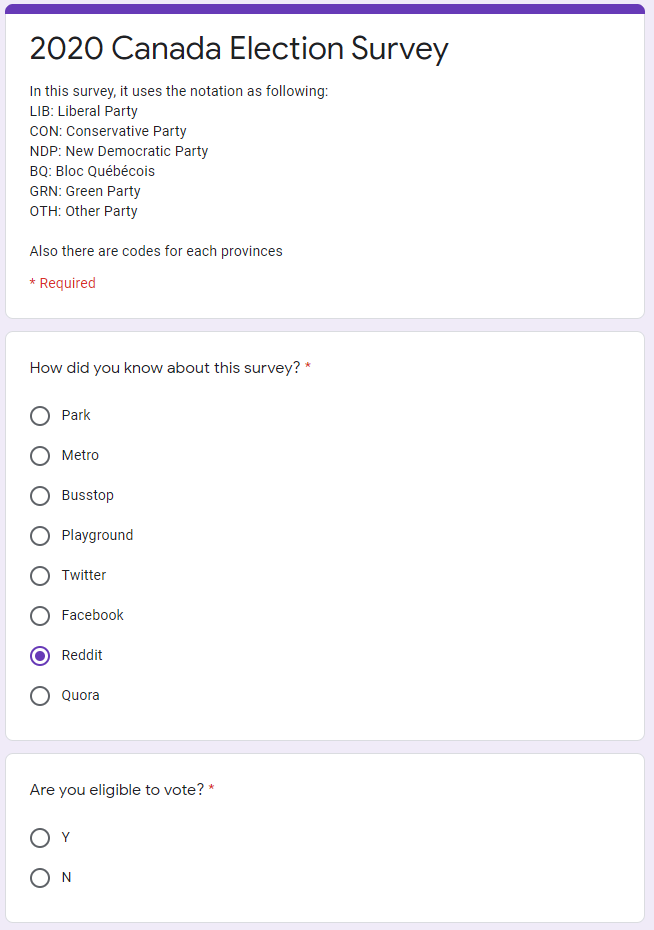
\includegraphics{./screenshot.PNG}
\caption{Screenshot}
\end{figure}

\end{document}
